\section{Einleitung}
Vor allem im 21. Jahrhundert wird Umweltfreundlichkeit immer wichtiger. Immer mehr Menschen fahren deshalb und aus vielen anderen Gründen (Gesundheit, Zeitersparnis, etc…) mit dem Fahrrad \cite{}. In vielen engen (und immer enger werdenden \cite{}) Großstädten der Welt ist das sichere Lagern von Fahrrädern jedoch schwierig bis unmöglich. Herkömmliche Fahrradständer sind zwar platzeffizient und billig, jedoch nicht sicher \cite{}. Besonders bei teuren E-Bikes traut sich mancher nicht, dieses einfach an einen Pfosten zu sperren. Als Alternative dazu gibt es Rad-Boxen oder unterirdische Garagen, beide Optionen sind aber teurer, eingeschränkt nutzerfreundlich und oft zu weit weg von dem Ort, an dem man hinwill.

\begin{figure}[ht]
  \centering
  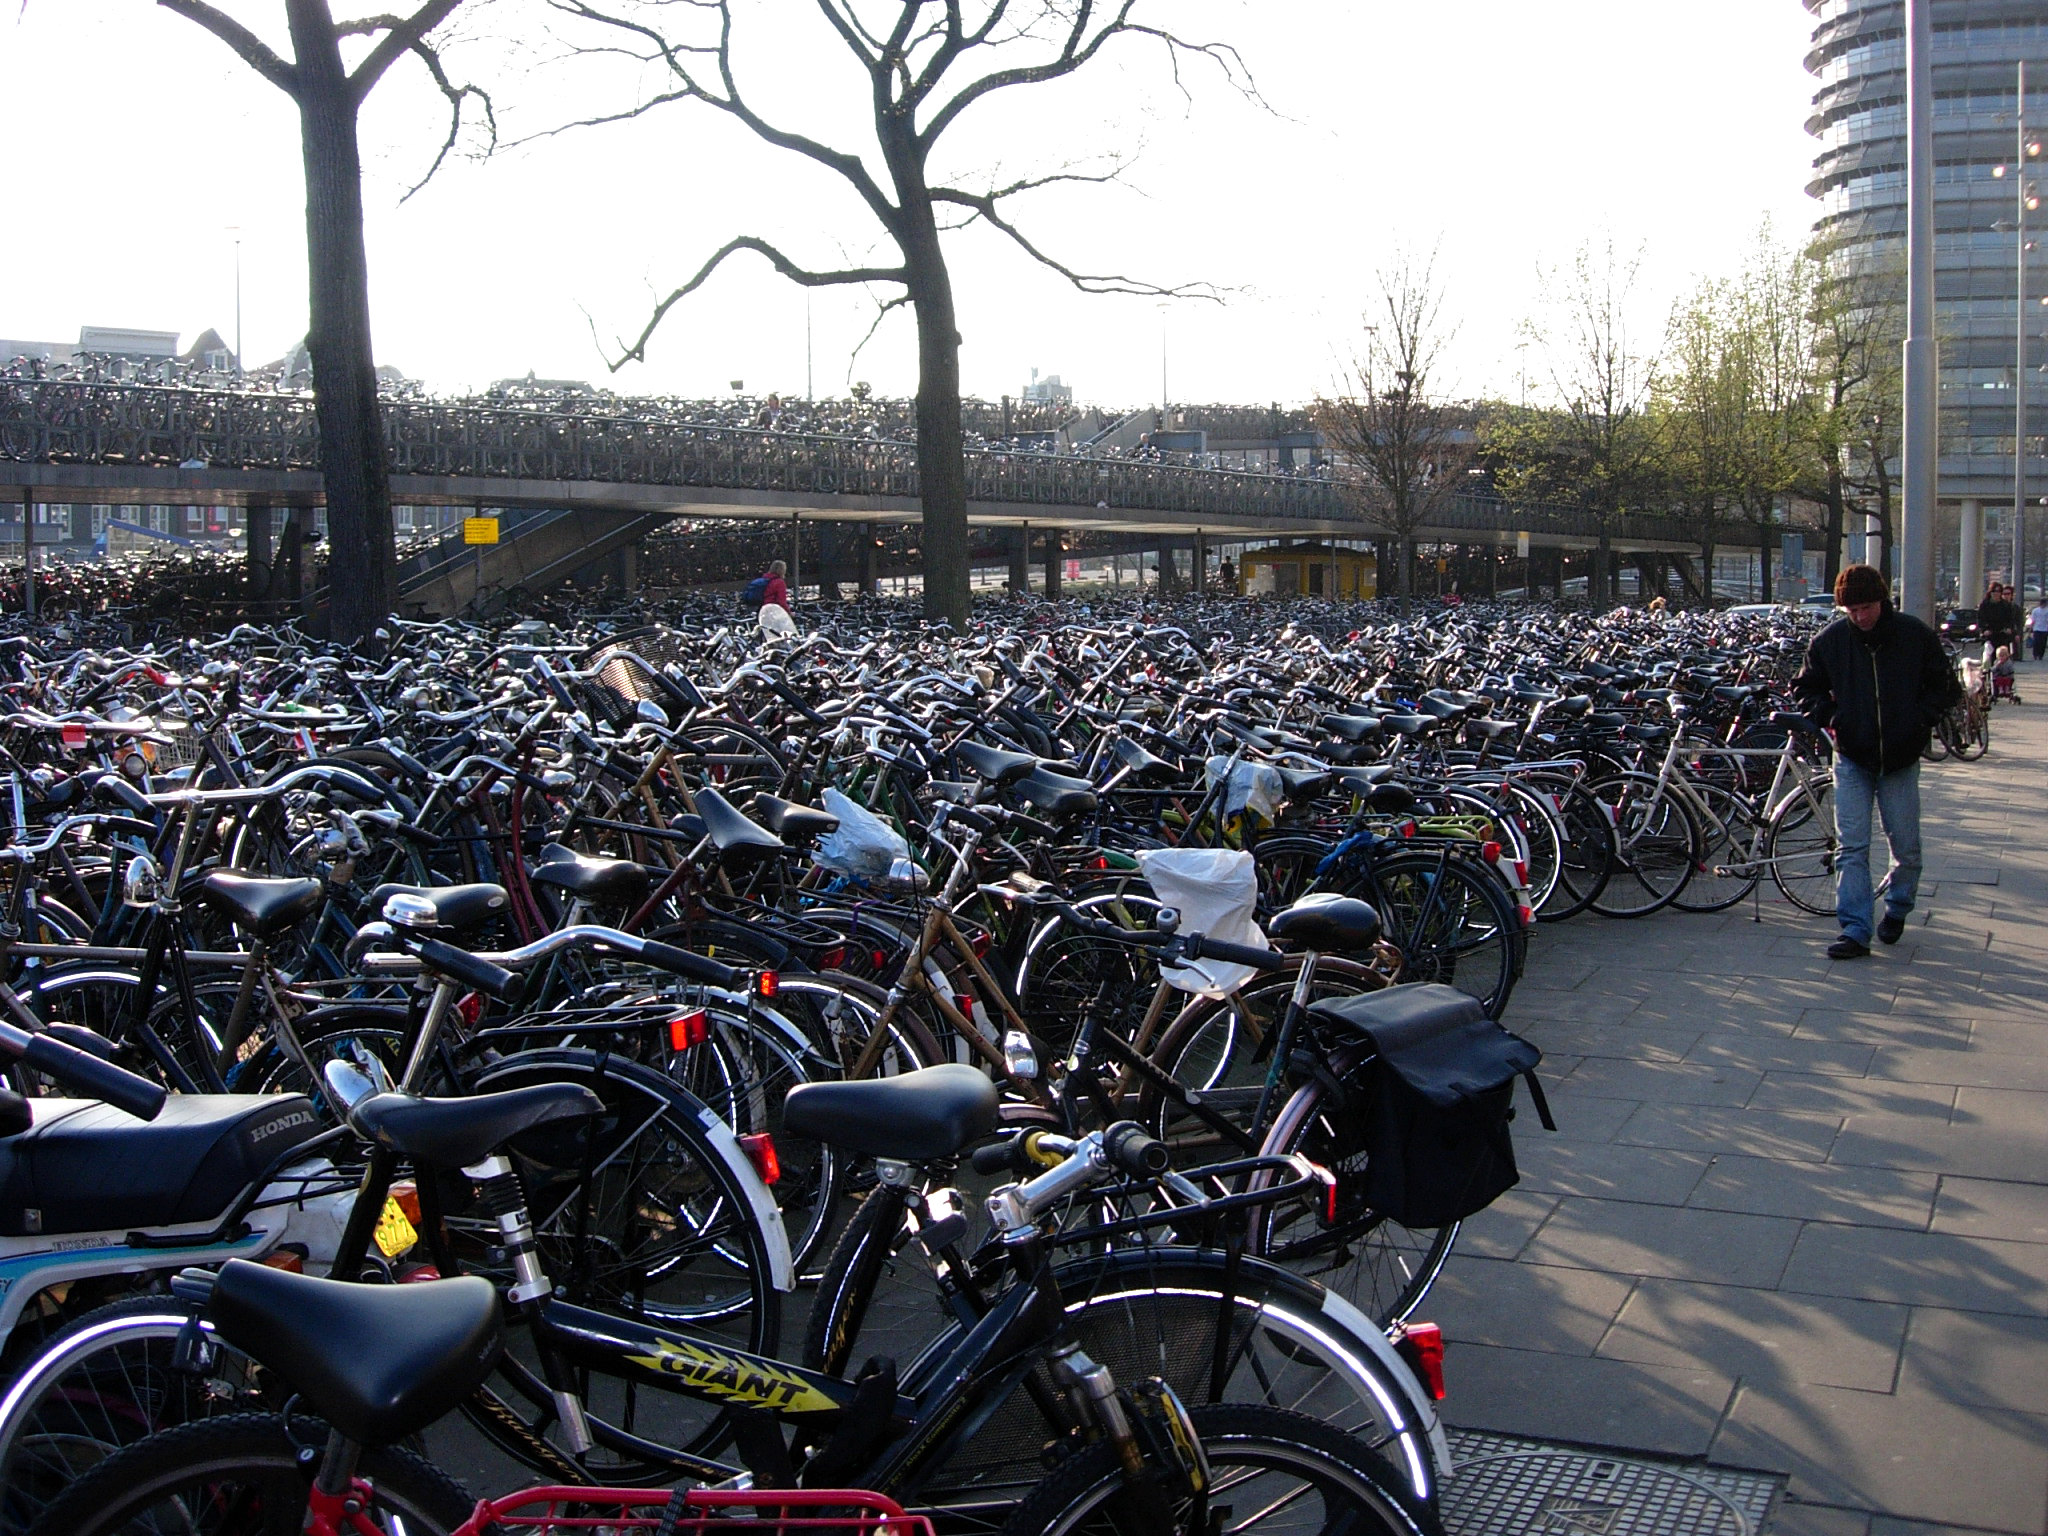
\includegraphics[width=0.5\textwidth]{images/fahrrad_parkhaus_voll}
  \caption{Randvolles Fahrrad-Parkhaus in Amsterdam (CC Jakub Hałun \cite{cc})}
  \label{fig:fahrrad_parkhaus_voll}
\end{figure}

In Zukunft wird es sogar noch mehr E-Bikes geben, denn fast die Hälfte aller verkauften Fahrräder sind mit Elektroantrieb ausgestattet (Tendenz stark steigend) \cite{}. Vor allem der urbane Raum benötigt derzeit dringend Abstellmöglichkeiten, wo Fahrräder schnell, sicher und möglichst billig in der Nähe geparkt werden können.

\subsection{Entstehung der Idee}

In Städten wie London oder Wien ist dem Projektbetreuer aufgefallen, dass immer mehr Stadtbewohner Fahrräder nutzen, es aber große Defizite bei sicheren Abstellplätzen gibt. Zuhause werden teure Fahrräder nicht selten auf die kleinen, wertvollen Balkone der Privatwohnungen (sicher) abgestellt. Einmal mit dem Fahrrad im stadtzentrum, wird es noch schwieriger. Das Projektteam vertritt die Hypothese, dass viele Stadtbewohner auf das Fahrrad umsteigen werden, sobald dieses Problem zufriedenstellen gelöst ist. Daraus formte sich die Idee eines „Fahrradturms“. Wie der Name schon verrät, ist ein Fahrradturm eine turmförmige Konstruktion, in der möglichst viele Fahrräder auf kleinstem Raum gelagert werden können. Die Vision sieht vor, die Fahrräder mittels automatischer Lagerroboter auf mehrere vertikalen Ebenen aufzuteilen, um die Platzeffizienz weiter zu steigern.

\begin{figure}[ht]
  \begin{center}
    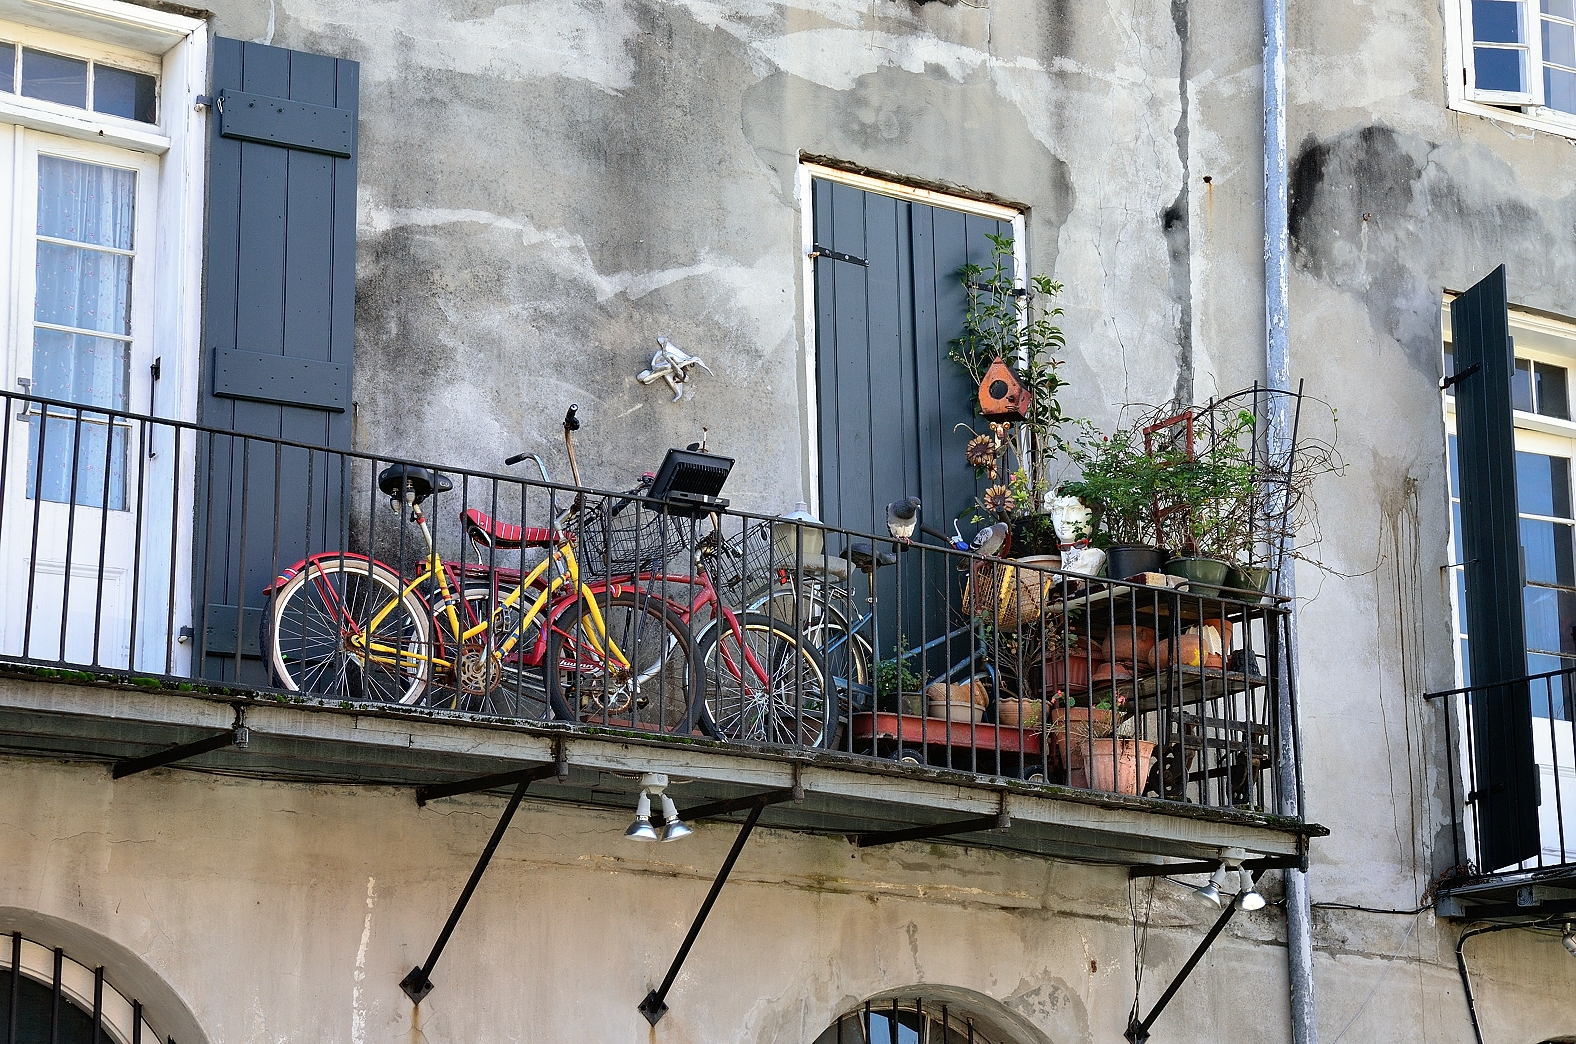
\includegraphics[width=0.5\textwidth]{images/fahrrad_balkon.jpg}
    \caption{Fahrradturm (CC Cliff Muller \cite{cc})}
    \label{fig:fahrrad_balkon}
  \end{center}
\end{figure}

\subsection{Zielsetzung}
Das Ziel ist die Entwicklung eines automatischen Fahrradparksystems zur effizienten, platzsparenden und sicheren Lagerung von Fahrrädern oder anderen Gegenständen an der Schnittstelle zum öffentlichen Verkehrsnetz. Es muss analysiert werden, welches System am ökonomischsten ist, unteranderem bei den Punkten Kosten, Flächenverbrauch und Nutzerfreundlichkeit, um anschließend ein Modell davon zu erstellen. Eine detaillierte technische Ausarbeitung ist nicht geplant. Schlussendlich ist geplant eine Softwarelösung für Benutzer (App) und ein Prototyp zur Veranschaulichung zu entwickeln.